\section{Context Awareness}
Software developers aim to build applications and systems that are easy to use. A way to accomplish this is to not only use data given by the user but also use context information from the users environment.

When a person talks to another person they are able to share specific information or context to increase the content of the conversation. The situation and the context makes it possible for a human to act according to this information. 
This ability is hard to transfer to human interaction with computers. Improving the computers ability to access and understand the circumstances developers can build context-aware applications that are easy to use. In order to understand what context-awareness is and where it is used, we first need to get a clear definition of context.
In earlier work Schilit and Thimer [10]is defining context as locations, identities of close people and objects. This definition is too specific. It's not only locations that is interesting as context. A better definition of context is:

\begin{quotation}
Context is a combination of any information that can be sensed or received by an entity which is useful to catch events and situations. Dey [9]
\end{quotation}

In other words context is information from an entity that gives specific information to increase the understanding of an events environment. An entity can be a person, place or a object that is interesting and relevant for the interaction. Smartphones is a good example of a device that gives a lot of context information because of the multiple sensors in the device. For example the sensors in a Google Nexus 4[6] are accelerometer, GPS, gyroscope, barometer, compass which can be used to collect context information about acceleration, location, velocity, rotation, pressure etc. This information can then be use to build context-aware applications. Context-awareness in applications will be more and more used nowadays when the concept Internet of things is growing. It's important for applications to take part of the context. When context is changing the applications need to handle the changes to fit the users interaction. Schmidt defines context-awareness in this way:

\begin{quotation}
Context-awareness is the ability of an entity to usefully adapt to or react based on context. 
\end{quotation}

Another definition of context-awareness is:

\begin{quotation}
A system is context-aware if it uses context to provide relevant information and\slash or services to the user, where relevancy depends on the user's task.
\end{quotation}

With these two definitions context-awareness means that we can use the context that is received by an entity and uses this information to interact with the application. An application is a context-aware application if it is able to use context in order to adjust its behaviour or the content it is providing. Example of context-awareness in applications is Google Latitude[7]. The application makes it possible for your friends to see your position on a map. Google Latitude uses the locations from a entity (mobile phone or computer) to update your position on the map. Another Context-aware application from google is AdSense\slash AdWords. This application generates advertisement based on the context of the webpage the user have visited. 
Also Android is a good example of context-awareness in application. When a user turns a smartphone or a tablet the operating system change 
it's orientation to landscape mode.

\begin{figure}[t]
	\centering
    	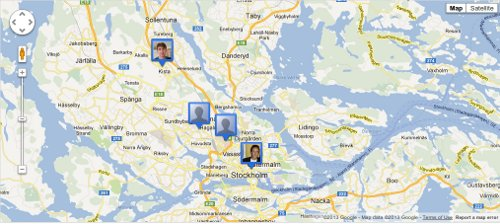
\includegraphics[scale=0.75]{part_2/context_awareness/latitude_pic.jpg}
		\caption{Figure text here} 
\end{figure}

\begin{figure}[t]
	\centering
    	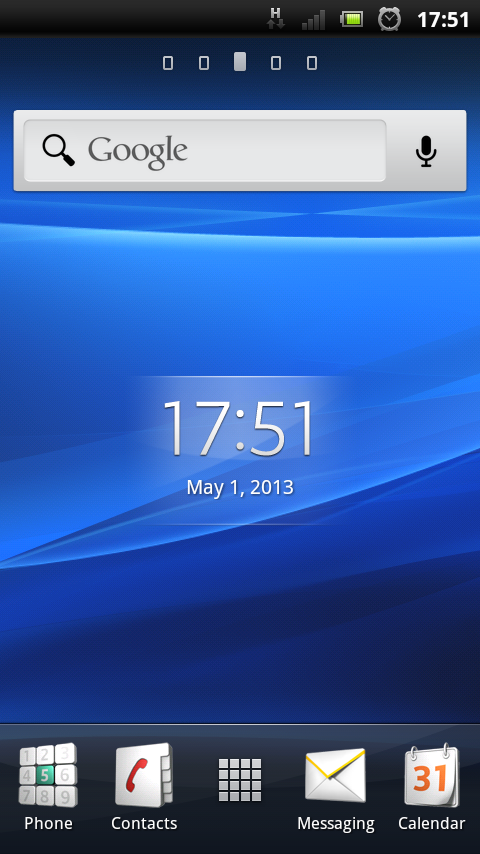
\includegraphics[scale=0.20]{part_2/context_awareness/screenshot_2013-05-01_1751.png}
    	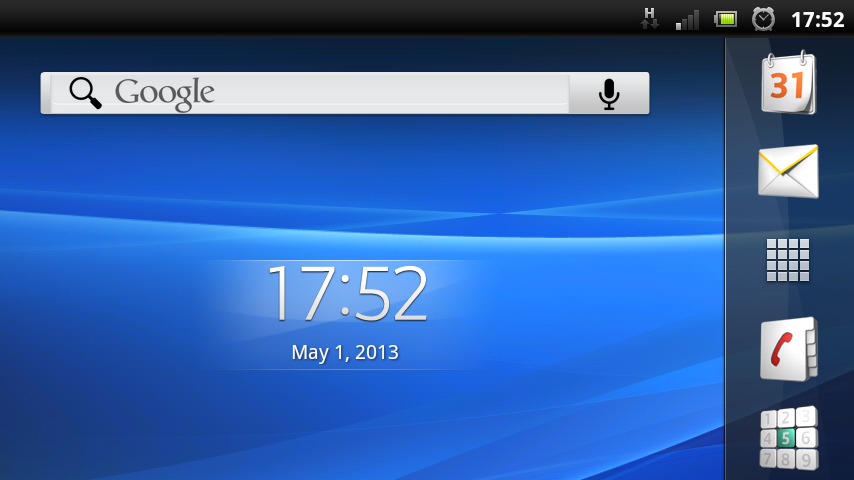
\includegraphics[scale=0.20]{part_2/context_awareness/screenshot_2013-05-01_1752.png}
		\caption{Figure text here} 
\end{figure}
	
A basic scenario of how a developer can build context\slash aware application is when the developer wants to create an application for turning on the light at home. The developer chooses to create the application without using context information. Then users will turn on lamps when pressing a button on the application. If the developer instead uses the context information the application can interact on information from sensors around the user. For example when a user enters his home the light will be turned on when the application detects his location from the users phone. The developer can also use information that provides how the weather is outside, if it's sunny outside the application will act to this and it will not turn on the lights when the user enters his home, but if it's cloudy outside the application will turn on the light.
